\section{General Analysis of Inventory Systems}
\label{sec:general}

\Opensolutionfile{ans}




% \subsection{Theory and Concepts}
% %\subsection*{Theory and Exercises}


Before making models of inventory systems we need to get an
understanding of the most relevant aspects of inventory systems. For
this purpose, lets start from the basics and see how far we get by
asking (relevant) questions. The most basic question is actually
'Why do we need inventory at all?', so that question will be our point
of departure.

\begin{exercise}
  Why do we need inventory at all?


\begin{solution}
\begin{enumerate}
\item Provide service (demand driven)
\begin{itemize}
\item uncertainty; e.g. demand, supply, production
\item capacity limitations in supply; production capacities, seasonal supply
\end{itemize}
\item Cost efficiency (operations driven)
\begin{itemize}
\item economies of scale; in procurement and transportation
\item speculation
\end{itemize}
\end{enumerate}
\end{solution}
\end{exercise}

\begin{exercise}
  When are inventory systems actually not necessary?


\begin{solution}
  In a sense, in business it comes down to matching supply and
  demand. When production capacity can be modulated at will and free of cost,
  there is not need for inventory. Any demand size be produced or
  ordered without any problem and without any financial consequence. The problem is of course that these two conditions are (nearly)
  never met in real systems.
\end{solution}
\end{exercise}


\begin{exercise}
When, then, are inventories necessary?


  \begin{solution}
    In real systems there are many constraints imposed on replenishing
    the inventory which makes matching supply and demand
    complicated.

    In case of \recall{Finished Goods Inventory} (\recall{FGI}), production limitations (production typically has     finite production speed, and works in batches because of setups),
    demand cannot be served when it arrives.  In case of \recall{Raw Materials Inventory} (\recall{RMI}), we need
    to respect supplier and transportation characteristics, so that we
    cannot order any quantity we like, and we need to take into
    account \recall{replenishment lead times}, which is the time between issuing an order at a supplier and the time receiving it. There can also be other
    constraints, for instance the supply can be only seasonable, e.g.,
    wheat.

    The items sold to customers has constraints such as the amounts in
    which it is produced, it can be perishable or not, and so on.

    The demand has constraints: customers may not be prepared to wait
    in \recall{backlog}, that is, they do not want to wait until their demand can satisfied.   It can actually be physically impossible to backlog
    demand. Finally, we can have \recall{lost sales}, i.e., demand that cannot be met right away from \recall{on-hand stock}, where stock on-hand means that the items are actually lying on a shelf. Thus, a certain  service level might need to be met.

    There are costs associated with all these constraints: ordering
    cost, holding cost, production costs, backlogging cost, lost
    sales, and so on.

    In this setting, with all these constraints, it is necessary to
    make trade-offs. Cost minimization then, typically, leads to
    installing inventories, since with inventories costs can be lower
    as compared to a system without an inventory. In fact, even if it technically possible to match supply and
    demand perfectly, there may be very high costs associated with the
    achieving this perfect match. Thus, in such cases, inventories are
    also used  to lower costs.
  \end{solution}
\end{exercise}

\begin{exercise}
Thus, all-in-all, what is the goal of an inventory system?


  \begin{solution}
    Inventory systems exist out of economic necessity. They are meant
    to provide a certain quality of service while reducing the cost of operations of a firm.
  \end{solution}
\end{exercise}


\begin{exercise}
  To put these ideas is a grand context, think about how the  three `buffers' \emph{inventory}, \emph{capacity}, and \emph{time} relate and can be traded against each other.
  \begin{solution}
    These three  buffers, \recall{inventory}, \recall{capacity}, and \recall{time}, are interrelated resources which can be used to satisfy demands. Suppose demand can be backlogged, that is, we do not have meet (all) demand from stock, but customers agree that (sometimes) they have to wait for their demand to be satisfied. Then, we need \emph{more} time, but  \emph{less} inventory to meet demand. We can also add capacity, as this typically shortens queueing time, that is, it shortens the time customers spend in backlog. Thus, by \emph{increasing} capacity, we can \emph{decrease} waiting time. Finally, if we have \emph{more} capacity, we can reduce intermediate inventories. All in all, the business context and the money will have a large influence on how we organize the production and inventory processes and how we deal with our customers. 
    
Note also that in case the inventory  is replenished by a production departurment (for instance a machine) with finite capacity, it may take some time to meet the backlog. Thus, in such capacitated inventory systems, backlogged demand  behaves  the same as the customers in a queue waiting for service. 

For a further, and highly  interesting, discussion, c.f., \cite[Chapter 6, Chapter 9]{hopp08:_factor_physic}. 
  \end{solution}
\end{exercise}

The core  of this course consists of developing and thinking about inventory models. This motivates the next question.

\begin{exercise}
Why is it important to make  models (from simple to difficult) of an inventory system?  
  \begin{solution}
    \begin{itemize}
    \item With a model it becomes possible to actually manage an
      inventory system. The model should include the basic, and most
      revelation, relations between the different parts of the system.
    \item A model can help with consistency checks. Suppose we estimate the cost of losing a demand as $10$ Euro. Assume also that we don't want to lose more than  $500$ Euro on loss per month. Thus, we don't want to lose more than $500/10=50$ customers per month. To ensure this, we need a certain amount of inventory on average. If this requirement, in turn, leads to absurdly high inventory, we either need to accept higher average loss costs, or our estimate of the cost of losing a demand, i.e., the $10$ Euro, is too high.  Typically, we cannot have it all: low inventory levels and no loss.

If we stick to the 10 Euro cost per loss customer, to the 500 Euro cost in total, and also to small on-hand inventory, we need to reorganize our production, or ordering, process.
    \item With models we can carry out simulations with the aim to
      evaluate the consequences of using certain types of control
      policies, i.e., \recall{when to order, and how much to order}.
    \item With models we can carry out sensitivity analysis. How
      sensitive is our policy with respect to changes in the cost
      parameters, demand, and so on? Suppose it turns out that the
      costs are very sensitive to certain parameters, then it may be important to monitor the
      inventory levels/positions closely. Or, we need to use other types, more robust control policies.
    \item Finally, we can use models for what-if scenarios.  We can
      investigate what happens if we change (some of) the assumptions
      underlying the model and develop methods to assess inventory
      control policies. With a model we can also analyze hypothetical
      situations and the efficacy of certain types of policies to
      avoid undesirable situations. (In fact, we use such models to
      try to understand how we can avoid ending up in a certain
      situation we never want to enter in reality.)
    \end{itemize}
  \end{solution}
\end{exercise}





When making a model of an inventory system, we first need to understand the environment.
The next questions address \emph{four} steps that can be used as a checklist, or guide, to characterize this environment. Of course, this list will not  be complete---it can never be complete, as inventory systems are much too varied---but it acts as a useful starting point.

\begin{exercise}
  What aspects are relevant to characterize the \emph{demand}?
  \begin{solution}
    To characterize demand the following questions are typically relevant.
      \begin{itemize}
      \item Can customers wait or not?  If so, how long? Is there a
        cost, like registration, associated with putting demand into
        backlog? Is there a cost associated with duration of waiting?
      \item Can demand be lost? If so, to what extent, e.g., 5\%? What
        is the cost of loss, or forgone revenue? 
      \item Is demand more or less constant or time-varying due to e.g. trends and seasonality?
      \item Is it deterministic or (very) stochastic? 
      \item Is it possible to use substitution to meet demand?
      \end{itemize}
  \end{solution}
\end{exercise}


\begin{exercise}
  What aspects are relevant to characterize the \emph{inventory system}?
\begin{solution}
 System characterization: 
      \begin{itemize}
      \item Characteristics of the replenishment structure and properties of items. 
      \item Are the inventories under \recall{continuous  review} (like the number of rice packets on the shelf in a supermarket, or the amount of gasoline at a tankstation), or under \recall{periodic review} (like the number of screws in a bucket).
      \item Are the items we sell produced or ordered, do we deal with a FGI or a RMI? 
      \item FGI:
      \begin{itemize}
      \item Can production be switched on and off?  Is there a cost
        associated with switching capacity on and off
      \item What is the production speed?
      \item Does production work in complete batches, or can it produce single items?
      \item Do we have to deal with MTO or MTS production? 
      \item Where to locate the I/O interface?
      \end{itemize}
    \item RMI:
      \begin{itemize}
      \item Is there a size constraint on the amount that can be ordered? 
      \item Is there a lead time between ordering and receiving the
        replenishment? Is the lead constant, variable, stochastic?
        Does it change over time?
      \item Is yield loss (i.e., we can not use all of the items that
        the supplier delivered) relevant ?
      \item Are orders always on time?
      \item Are items ordered jointly with other items, joint
        replenishments?
      \item Is there a cost associated with ordering? Is there a fixed
        and/or and variable part of this cost? Quantity discounts?
      \item How many suppliers do we have?
      \end{itemize}
    \item Items:
      \begin{itemize}
      \item Are items held at one single-echelon, or in a multi-echelon system?
      \item Are the items perishable or not? Is there a cost associated with deterioration?
      \item Are we concerned with ordering just one item type or more? In case of the latter, can orders be joined or not? 
      \item What are the costs associated with holding inventories?
      \item Are there budget and/or warehouse limitations?
      \item Are we dealing with \recall{Make to Order} (\recall{MTO}) items, or \recall{Make to Stock} (\recall{MTS}) items? Would it be a good idea to move MTS items to MTO (or the other way around?) If there is just sporadic demand, MTO might be desirable. However, we might be dealing with spare parts. In such cases, we cannot wait to make the needed items; MTS is then the logical choice, even though it is expensive. 
      \item More in general, when designing the inventory system, where should we put the \recall{Inventory/Order} (\recall{I/O}) point? Here, upstream of the I/O interface, we typically produce as MTS, and downstream as MTO. Observe, not all items need to have their  I/O interface at the same position in the production-inventory system or supply chain.. 
 \end{itemize}
\end{itemize}
\end{solution}
\end{exercise}

\begin{exercise}
  What aspects are relevant to select an \emph{inventory policy}?
\begin{solution}
 Policy selection:
      \begin{itemize}
      \item What do we want to achieve? Satisfy a service level
        constraint, or minimize cost? In case of the latter, do we
        want to minimize cost over one or many periods? What are the relevant KPIs? 
      \item Periodic or continuous review?
      \item What decisions/controls are at our disposal to affect the
        behavior of the system, hence affect the cost?
      \item What properties do we require? Should it be simple?
        Operate it manually, or by computer? 
      \end{itemize}
See the figure below for a (quite outdated) visual overview of inventory models in the literature.

%\begin{figure}[h]
\centering
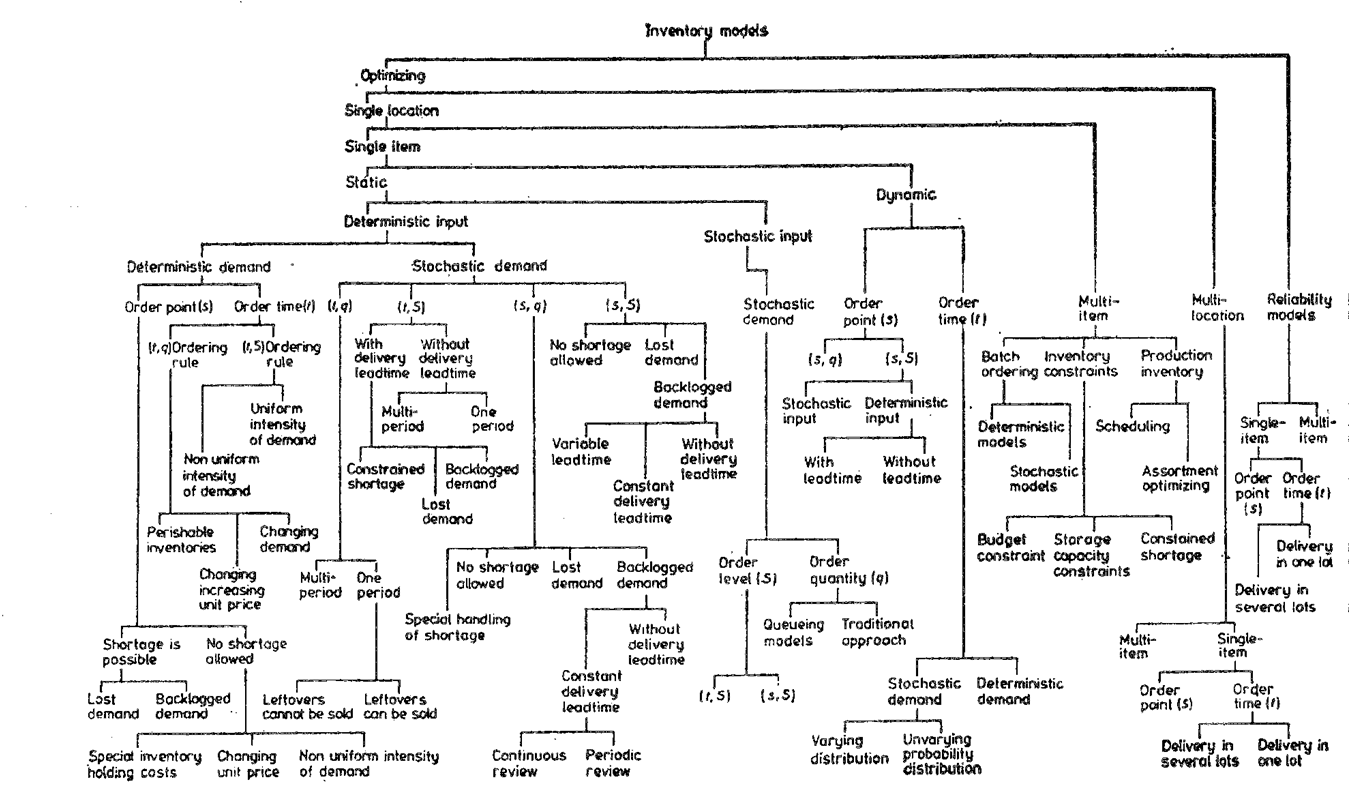
\includegraphics[width=\textwidth]{figures/chikan.png}
%\caption{Decomposition of inventory models}
%\label{fig:costs}
%\end{figure}
    \end{solution}
  \end{exercise}
  

\begin{exercise}
  What aspects are relevant to evaluate the performance of the \emph{inventory policy}?
\begin{solution}
Policy evaluation:
      \begin{itemize}
      \item What customer service level do we need, e.g., fill rate, cycle-service level? What are the importance of different KPI's?
      \item What weight  should we assign to the relevant cost components; which is most important, which are less important?
      \item How can we find good (near-optimal) policy parameters once we have chosen for a certain policy?
      \end{itemize}

  \end{solution}
\end{exercise}


% \begin{exercise}
% In the case of constant and continous demand, it is a bit hard to give an interpretation to the cost parameter $\pi$. Why?
%   \begin{solution}
% The cost $\pi$ counts cost per incoming customer. When demand is continuous, there is no such thing as a single customer.  Only when     demand enters in discrete amounts, we should include backlog cost $\pi$ per demand. 
%   \end{solution}
% \end{exercise}

In the remainder of these notes we'll use the checklist we developed in the above exercises to model and analyze the inventory systems. We'll make a model first, with symbols, because this helps in the communication about the model and the documentation. Once we have a complete model we can
implement  it in some computer system (spreadsheet or programm), simulate it and evaluate
the efficacy of inventory control policies.  

Note that modeling is an art; as a consequence, checklists can never be
complete, and there is also not one simple recipe to make a good
model. In that sense, the development of models is always somewhat
ad-hoc and unstructured, in fact, the development of the model helps
you to familiarize yourself with a situation you don't completely
understand. There is no way around except that you start modeling,
accept to make mistakes in the process, and test your assumptions and
modeling decision, improve your model after these tests, and so on. The
proof of the pudding is in the eating\ldots and you don't know upfront
whether your model will be correct or not.\footnote{For the interested, we refer to \cite[Section 2.1, 2.2, 6.3 and 16.2.]{hopp08:_factor_physic}.}


\Closesolutionfile{ans}
\opt{solutionfiles}{
\subsection{Solutions}
\input{ans}
}


\clearpage
%%% Local Variables:
%%% mode: latex
%%% TeX-master: "inventory_notes"
%%% End:
